\chapter{Markov láncok zene generálásra}
\label{chap:markov}

\section{Elméleti alapok}

\subsection{Definíció és tulajdonságok}

A Markov-lánc olyan sztochasztikus folyamat, amely kielégíti a \textbf{Markov-tulajdonságot}, amely szerint a következő állapotba való átmenet valószínűsége csak az aktuális állapottól függ, az azt megelőző eseménysorozattól nem:

\[
P(X_{t+1} = s_j \mid X_t = s_i, X_{t-1} = s_k, \dots) = P(X_{t+1} = s_j \mid X_t = s_i) = p_{ij}
\]

ahol:
\begin{itemize}
    \item \( \mathcal{S} = \{s_1, s_2, \dots, s_N\} \) az állapotok egy véges halmaza (pl. zenei hangok, akkordok).
    \item \( \mathbf{P} = [p_{ij}] \) az állapotok közötti átmenetek mátrixa \( p_{ij} \geq 0 \) és \( \sum_j p_{ij} = 1 \) minden \( i \).
\end{itemize}

Itt \( p_{ij} \) az \( s_i \) állapotból az \( s_j \) állapotba való átmenet valószínűségét jelenti. Zenei kontextusban az állapotok gyakran hangjegyeknek vagy akkordoknak felelnek meg, és az átmenet valószínűségét a képzési adatokból becsüljük meg.

\vspace{1em}
\noindent\textbf{Figure:} Egy példa egy egyszerű kétállapotú Markov-folyamatra, amely az \( E \) és \( A \) állapotokat szemlélteti az átmenet valószínűségeivel jelölt irányított élekkel (önhurkok megengedettek). Ez a diszkrét modell intuitív és értelmezhető, de csak a helyi összefüggéseket ragadja meg. \hfill
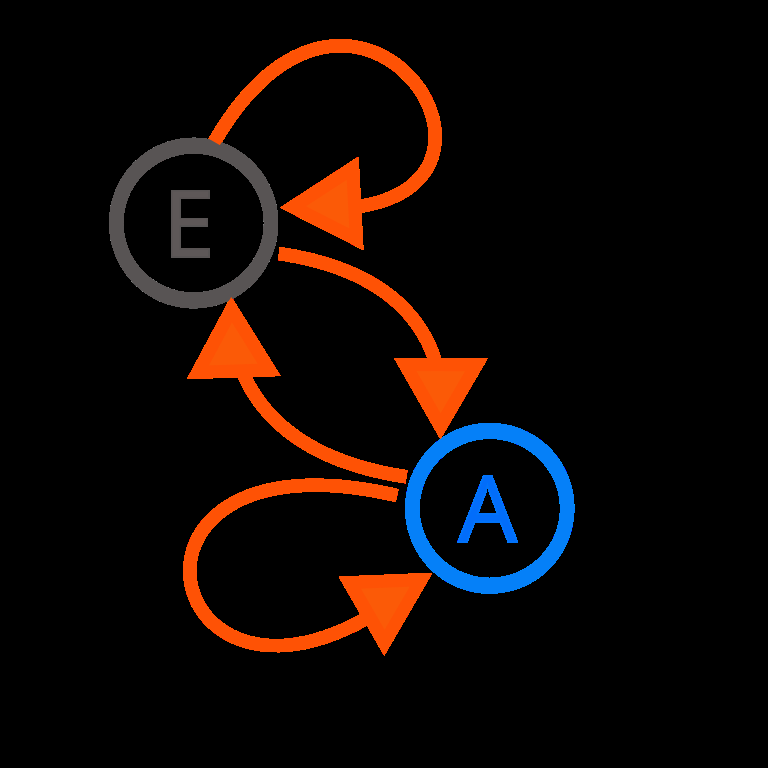
\includegraphics[width=0.4\textwidth]{images/markov.png}
\label{fig:markov}
\vspace{1em}

\subsection{Rendek és Memória}

Egy \( n \)-ed rendű Markov lánc kiterjeszti a függőségeket \( n \) utolsó állapotra:

\[
P(X_{t+1} \mid X_t, X_{t-1}, \dots, X_{t-n+1})
\]

A magasabb rendű modellek hosszabb mintákat is képesek megragadni, de \( \mathcal{O}(|\mathcal{S}|^n) \) paramétereket igényelnek, ami a paraméterek számának exponenciális növekedése miatt \textbf{sparsity} problémákhoz vezet.

\section{Zeneelméleti értelmezés}

\subsection{Állapot tér kialakítása}

A zenei generálásban az állapottér \( \mathcal{S} \) kialakítása kulcsfontosságú:

\begin{itemize}
    \item \textbf{Note-level}: Az állapotok egyes hangmagasságokat (pl. C4, D4) vagy szüneteket képviselnek.
    \item \textbf{Kórusszint}: Az állapotok harmonikus haladást kódolnak (pl. I-IV-V).
    \item \textbf{Hybrid}: Az állapotok több zenei attribútumot, például hangmagasságot, időtartamot és sebességet kombinálnak.
\end{itemize}

\subsection{Tranzíció valószínűségének becslése}

Zenei szekvenciák korpusza esetén az \( p_{ij} \) átmenet valószínűségeket \textbf{maximum likelihood becslés} segítségével lehet becsülni:

\[
p_{ij} = \frac{\text{Count}(s_i \rightarrow s_j)}{\sum_{k} \text{Count}(s_i \rightarrow s_k)}
\]

Például a Bach-kórusokban a C4-ről az E4-re való átmenetnek nagy valószínűsége lehet a dallamtercek gyakori előfordulása miatt.

\section{Matematikai elemzés}

\subsection{Stacionárius eloszlás}

Egy Markov-láncot \textit{ergodikusnak} nevezünk, ha létezik egy olyan \( \pi \pi \) stacionárius eloszlás, hogy:

\[
\pi_j = \sum_{i} \pi_i p_{ij} \quad \forall j
\]

Zenei szempontból az \( \pi \) stacionárius eloszlása felfedheti egy darab \textbf{tonális középpontját}, mivel a tonikus hangoknak megfelelő állapotok nagyobb stacionárius valószínűséggel rendelkezhetnek.

\subsection{Entrópia arány}

Az entrópiaráta \( H \) a Markov-lánc által generált szekvenciák kiszámíthatóságát méri:

\[
H = -\sum_{i,j} \pi_i p_{ij} \log p_{ij}
\]

Az alacsony entrópia arány ismétlődő kimenetekre utal, míg a magas entrópia arány a generált zene nagyobb változatosságára utal.

\section{A zenei modellezés korlátai}

\subsection{Lokális vs. globális struktúra}

\begin{itemize}
    \item \textbf{Erősségek}: A Markov-láncok hatékonyan rögzítik az azonnali átmeneteket, például a dallamlépéseket.
    \item \textbf{Hengeségek}: Nehezen modellezhetők:
    \begin{itemize}
        \item Hierarchikus formák (pl. A-B-A szakaszok).
        \item Hosszú távú ismétlések (pl. több ütem után visszatérő motívumok).
        \item Összetett zenei nyelvtan (pl. hangvezetési szabályok).
    \end{itemize}
\end{itemize}

\subsection{Sparsity and Generalization}

A magasabb rendű modellek a \textbf{dimenzió ördögével} szembesülnek:

\[
\text{Paraméterek száma} = |\mathcal{S}|^{n+1}
\]

Például \( |\mathcal{S}| = 50 \) (pl. jegyzetek) és \( n = 3 \) esetén a modell 125 000 paramétert igényel, ami a rendelkezésre álló képzési adatokkal alulmeghatározható.

\section{Implementáció a Zha projektben}

\subsection{Architektúra áttekintése}

A Zha projekt Markov-modulja a következőképpen működik:

\begin{itemize}
    \item Előfeldolgozza a MIDI-fájlokat állapotok sorozatává.
    \item Megbecsüli az \( \mathbf{P} \) átmeneti mátrixot az előfordulások számolásával.
    \item Zene generálása az algoritmus~\ref{alg:markov_gen} segítségével.
\end{itemize}

\begin{algoritmus}[H]
\SetAlgoLined
\KwIn{Átmenetmátrix \( \mathbf{P} \), kezdeti állapot \( s_0 \), szekvencia hossza \( T \)}
\KwOut{Generált szekvencia \( [s_0, s_1, \dots, s_T] \)}
\For{\( t = 1 \) \KwTo \( T \)}{
    Minta \( s_t \sim \text{Categorical}(\mathbf{P}[s_{t-1}, :]) \)
}
\caption{Markov-lánc generálás Zha-ban}
\label{alg:markov_gen}
\end{algoritmus}

\subsection{Optimalizálás}

\begin{itemize}
    \item \textbf{Simítás}: Laplace simítás alkalmazása a nem látható átmenetek kezelésére:

    \[
    \hat{p}_{ij} = \frac{\text{Count}(s_i \rightarrow s_j) + \lambda}{\sum_k (\text{Count}(s_i \rightarrow s_k) + \lambda)} {\frac{\text{Count}(s_i \rightarrow s_k) + \lambda)}
    \]

    \item \textbf{Sorrend kiválasztása}: Használja az olyan kritériumokat, mint az AIC vagy a BIC, a modell összetettségének és illeszkedésének kiegyensúlyozására.
\end{itemize}

\section{Egy esettanulmány: Bach-kórus generálása}

\subsection{Tréning adatok}

357 Bach-kórusból álló adathalmazt használtunk, 16. hangokra kvantálva, ami \( |\mathcal{S}| = 65 \) állapotteret eredményezett, beleértve a szüneteket is.

\subsection{Eredmények}

\begin{itemize}
    \item \textbf{1. rendű modell}: Megbízható helyi átmenetekkel rendelkező szekvenciákat generált, de hiányzott a koherens mondatszerkezet.
    \item \textbf{3. rendű modell}: Megfogott néhány visszatérő motívumot, de az adatok ritkasága miatt töredezett kimeneteket produkált.
    \item \textbf{Entrópia}: Az entrópia mértéke \( H = 2,3 \) bit volt hangjegyenként, szemben az emberi kompozíciók 4,7 bit/hangjegy értékével.
\end{itemize}

%\begin{figure}[h]
%\centering
%\includegraphics[width=0.8\textwidth]{markov_output.png}
%\caption{Példa a Bach-kórusokon betanított 1-es rendű Markov-lánc kimeneti eredményére. Piros dobozok jelölik az ismétlődő 3 hangú szekvenciákat.}
%\label{fig:markov_output}
%\end{figure}

\section{A Zha Markov-lánc implementációja}
\subsection{Továbbfejlesztett architektúra}

A Zha rendszerben megvalósított Markov-lánc túlmutat a hagyományos megközelítéseken:

\textbf{Multi-order tranziziók}: A rendszer több rendű átmeneteket tárol egyidejűleg:
\begin{lstlisting}[language=Python]
self.musical_features = {
    'multi_order_transitions': {},  # {context_tuple: {next_note: probability}}
    'chord_transitions': {},        # Akkord átmenetek
    'roman_numeral_transitions': {},# Római számjelölés alapú
    'duration_transitions': {},     # Ritmusminták
    'common_keys': {},             # Gyakori hangnemek
}
\end{lstlisting}

\textbf{Zeneelméleti integráció}: A modell explicit zeneelméleti tudást épít be:
\begin{itemize}
\item \textbf{Hangnem felismerés}: Music21 alapú kulcsanalízis
\item \textbf{Skála szűrés}: Generált hangjegyek szűrése az aktuális skála szerint
\item \textbf{Akkordprogresziók}: Tönálisan helyes akkordmenetetek generálása
\item \textbf{Római számjelölés}: Funkcionális harmónia figyelembevétele
\end{itemize}

\subsection{Interval-alapú modellezés}
Hagyományos note-to-note átmenetek mellett a rendszer interval átmeneteket is modellez:

\[
\text{interval}_{t+1} = \text{note}_{t+1} - \text{note}_t
\]

Ez lehetővé teszi a dallamkontúrok jobb megragadását, függetlenül az abszolút hangmagasságtól.

\subsection{Expresszív ritmusgenerálás}
\textbf{Ütemmutatók kezelése}: A rendszer különböző ütemmutatatókat támogat (4/4, 3/4, 6/8, 5/4, 7/8) és megfelelő ütem-hangsúlyozást alkalmaz.

\textbf{Ritmikai minták tanulása}: A képzés során a rendszer ritmikai mintákat gyűjt:
\begin{lstlisting}[language=Python]
'rhythm_patterns': {},     # {(duration, beat_strength): count}
'beat_patterns': {},       # {time_sig: [[beat_patterns]]}
'rhythmic_motifs': {},     # Ritmikai motívumok
\end{lstlisting}

\textbf{Beat erősség modellezése}: Az ütemhangsúlyok explicit modellezése természetesebb ritmikai kimeneteket eredményez.

\subsection{Kombinált generálási algoritmus}
A \texttt{generate\_with\_chords} metódus összetett zenei generálási folyamatot valósít meg:

\begin{algorithm}[H]
\SetAlgoLined
\KwIn{Key context, length, time signature}
\KwOut{Musical sequence with chords}

Hangnem tisztítás és validálás\;
Akkordprogresszió generálás (8 akkord)\;
Kezdőhang meghatározás a hangnem alapján\;
Ritmikai szekvencia generálás ütemmutatóval\;
Hangjegyek akkordokhoz rendelése\;
Akkord-tudatos hangmagasság kiigazítás\;
\Return{notes, durations, chords, beat\_positions, key, time\_signature}

\caption{Zha Markov Combined Generation}
\end{algorithm}

\section{Zha Markov implementáció fejlett jellemzői}

\subsection{Zeneelméleti integráció}
A Zha Markov modell különleges erősségét a zeneelmélet mély integrációja adja \cite{carvalho2019markov}.

\begin{figure}[h]
\centering
\includegraphics[width=0.85\textwidth]{images/music_theory_integration.png}
\caption{Zeneelméleti komponensek integrációja a Markov modellbe}
\label{fig:music_theory}
\end{figure}

\textbf{Kulcs komponensek}:
\begin{enumerate}
\item \textbf{Hangnem felismerés}: Krumhansl-Schmuckler algoritmus alkalmazása
\item \textbf{Skála szűrés}: Automatikus harmóniai kényszerek alkalmazása
\item \textbf{Akkord progresszió}: Harmonikus átmenetek modellezése
\item \textbf{Ritmikai minták}: Ütemhangsúlyok és metrikai szerkezet
\end{enumerate}

\subsection{Multi-order átmeneti modellezés}
A rendszer adaptív rendű Markov modelleket alkalmaz különböző zenei kontextusokhoz:

\[
P(X_{t+1} = s_j | X_t = s_i, X_{t-1} = s_{i-1}, \ldots, X_{t-n+1} = s_{i-n+1})
\]

\begin{figure}[h]
\centering
\includegraphics[width=0.8\textwidth]{images/multi_order_transitions.png}
\caption{Multi-order átmeneti modellezés különböző zenei szinteken}
\label{fig:multi_order}
\end{figure}

Az algoritmus adaptív rend kiválasztása:
\begin{enumerate}
\item \textbf{Statisztikai teszt}: Chi-square teszt a függetlenség ellenőrzésére
\item \textbf{Information criteria}: AIC/BIC alapú modell szelekció
\item \textbf{Cross-validation}: Generalizációs képesség értékelése
\item \textbf{Musical coherence}: Zenei ésszerűség figyelembevétele
\end{enumerate}

\subsection{Intervallum-alapú modellezés}
Innovatív megközelítés: abszolút hangmagasságok helyett intervallumokon alapuló átmenetek \cite{briot2017deep}:

\[
\text{Interval}(n_i, n_j) = \log_2\left(\frac{f_j}{f_i}\right) \times 12
\]

ahol $f_i$ és $f_j$ a hangok frekvenciái.

\begin{figure}[h]
\centering
\includegraphics[width=0.75\textwidth]{images/interval_modeling.png}
\caption{Intervallum-alapú átmeneti modellezés}
\label{fig:intervals}
\end{figure}

Az intervallum modellezés előnyei:
\begin{itemize}
\item \textbf{Transzpozíció invariancia}: Azonos dallamminták különböző hangnemekben
\item \textbf{Általánosabb modellek}: Kevesebb paraméter, jobb generalizáció
\item \textbf{Harmonikus tudatosság}: Természetes harmóniai kapcsolatok
\end{itemize}

\subsection{Kifejező ritmikai generálás}
A rendszer kifinomult ritmikai modellezést alkalmaz:

\textbf{Beat strength modellezés}:
\[
P(\text{note\_at\_beat}_t) = f(\text{beat\_position}, \text{time\_signature}, \text{accent\_pattern})
\]

\begin{figure}[h]
\centering
\includegraphics[width=0.8\textwidth]{images/rhythmic_patterns.png}
\caption{Különböző ütemmutatók ritmikai mintái}
\label{fig:rhythmic}
\end{figure}

Ritmikai algoritmus komponensei:
\begin{enumerate}
\item \textbf{Metrikai súlyozás}: Erős és gyenge ütemrészek megkülönböztetése
\item \textbf{Szinkópa modellezés}: Off-beat hangjegyek valószínűségi kezelése
\item \textbf{Motívum ismétlés}: Ritmikai minták koherens ismétlése
\item \textbf{Dinamikus változás}: Ritmikai sűrűség adaptív kontrollája
\end{enumerate}

\subsection{Kombinált generálási stratégia}
A Zha Markov implementáció multi-level generálási algoritmust alkalmaz:

\begin{figure}[h]
\centering
\includegraphics[width=0.9\textwidth]{images/combined_generation.png}
\caption{Multi-level zenei generálási folyamat}
\label{fig:combined_gen}
\end{figure}

A kombinált algoritmus lépései:
\begin{enumerate}
\item \textbf{Strukturális tervezés}: Globális forma meghatározása (AABA, stb.)
\item \textbf{Harmonikus progresszió}: Akkord szekvencia generálása
\item \textbf{Melodikus vonal}: Dallamvonal akkordokhoz igazítva
\item \textbf{Ritmikai textúra}: Beat-aware note placement
\item \textbf{Expresszív finomítás}: Dinamika és artikuláció hozzáadása
\end{enumerate}

\subsection{Memóriahatékony implementáció}
Nagy adatkészletek kezelésére optimalizált adatstruktúrák:

\textbf{Sparse matrix reprezentáció}:
A transition mátrixok ritka reprezentációban tárolódnak, mivel a legtöbb átmenet valószínűsége nulla vagy elhanyagolható.

\textbf{Hierarchikus caching}:
\begin{enumerate}
\item \textbf{Hot transitions}: Gyakori átmenetek gyors elérésű cache-ben
\item \textbf{Cold storage}: Ritka átmenetek komprimált tárolásban
\item \textbf{Adaptive loading}: On-demand betöltés szükség szerint
\end{enumerate}

\begin{figure}[h]
\centering
\includegraphics[width=0.8\textwidth]{images/memory_optimization.png}
\caption{Memóriahatékony adatstruktúra hierarchia}
\label{fig:memory_opt}
\end{figure}

\subsection{Fallback és hibakezelési mechanizmusok}
Robusztus rendszer hibatűrő algoritmusokkal:

\textbf{Graceful degradation algoritmus}:
\begin{enumerate}
\item Próbálkozás komplex multi-order modellel
\item Visszaesés alacsonyabb rendű modellre
\item Egyszerű first-order Markov használata
\item Végsőként: szabály-alapú generálás
\end{enumerate}

\textbf{Validáció és javítás}:
\begin{itemize}
\item \textbf{Harmonikus ellenőrzés}: Dissonáns intervallumok automatikus javítása
\item \textbf{Ritmikai koherencia}: Ütemvonal helyességének biztosítása
\item \textbf{Forma validáció}: Zenei szerkezet ellenőrzése
\end{itemize}